\documentclass[11pt,a4paper]{article}
\usepackage{amsmath}
\usepackage{amssymb}
\usepackage{geometry}
\usepackage{graphicx}
\usepackage{hyperref}
\usepackage{booktabs}
\usepackage{bm}
\usepackage{float}
\usepackage{tikz}
\usetikzlibrary{arrows.meta, positioning, shapes.geometric, calc}

\geometry{margin=1in}

\title{Vehicle Dynamics with Dugoff Tire Model}
\author{Mario Tilocca}
\date{January 2026 -- Version 2.0}

\begin{document}

\maketitle


\begin{abstract}
This document presents the transition from a kinematic bicycle model to a dynamic vehicle model incorporating the Dugoff tire model with wheel rotational dynamics. We derive the complete force-based dynamics, normal load distribution with load transfer, slip ratio computation, friction-limited tire forces, and wheel angular velocity integration. The hybrid torque-slip model enables realistic simulation of traction limits, wheel spin, wheel lock, and combined longitudinal-lateral dynamics for autonomous mining haul truck applications.
\end{abstract}


\tableofcontents
\clearpage


%=============================================================================
\section{Introduction}
%=============================================================================

\subsection{Motivation for Dynamic Model}

The kinematic bicycle model assumes:
\begin{itemize}
    \item \textbf{No slip:} Pure rolling condition at all times
    \item \textbf{Unlimited traction:} Tire forces can be arbitrarily large
    \item \textbf{Instantaneous response:} No force buildup dynamics
\end{itemize}

These assumptions break down when:
\begin{itemize}
    \item Vehicle operates on low-friction surfaces (gravel, wet haul roads)
    \item Emergency braking or aggressive acceleration
    \item Combined maneuvers (braking while turning)
    \item Realistic traction control and ABS simulation required
\end{itemize}

The Dugoff tire model addresses these by:
\begin{itemize}
    \item Computing friction-limited forces based on normal load
    \item Modeling slip ratios (longitudinal and lateral)
    \item Capturing smooth saturation from linear to sliding regimes
\end{itemize}

\subsection{Model Architecture Evolution}

We present three levels of modeling fidelity:

\textbf{Kinematic Model (V1):}
\begin{equation}
\text{Actuator} \to \text{Drive} \to \text{Velocity} \to \text{Position/Yaw}
\end{equation}

\textbf{Torque-Only Dynamic Model (V2):}
\begin{equation}
\text{Actuator} \to \text{Drive} \to \boxed{\text{Tire Forces (friction-limited)}} \to \text{Acceleration} \to \text{Velocity}
\end{equation}

\textbf{Hybrid Torque-Slip Model (V2.5):}
\begin{equation}
\text{Actuator} \to \boxed{\text{Wheel Dynamics}} \to \boxed{\text{Slip}} \to \boxed{\text{Dugoff Forces}} \to \text{Vehicle Dynamics}
\end{equation}

The hybrid model adds wheel rotational dynamics, enabling natural slip development, wheel spin, and wheel lock simulation.

\subsection{Model Comparison Summary}

\begin{table}[H]
\centering
\begin{tabular}{lccc}
\toprule
\textbf{Feature} & \textbf{Kinematic} & \textbf{Torque-Only} & \textbf{Hybrid} \\
\midrule
Traction limit & Unlimited & $\mu F_z$ & $\mu F_z$ \\
Wheel slip & None & Estimated & Computed \\
Wheel spin & No & No & Yes \\
Wheel lock & No & No & Yes \\
TCS/ABS testing & No & Limited & Full \\
Computational cost & Low & Low & Medium \\
\bottomrule
\end{tabular}
\caption{Tire model comparison}
\end{table}

%=============================================================================
\section{Force-Based Longitudinal Dynamics}
%=============================================================================

\subsection{Equations of Motion}

Newton's second law in the longitudinal direction:
\begin{equation}
m \frac{dv}{dt} = \sum F_x - F_{\text{drag}} - F_{\text{roll}}
\end{equation}

where:
\begin{align}
\sum F_x &= F_{x,\text{fl}} + F_{x,\text{fr}} + F_{x,\text{rl}} + F_{x,\text{rr}} \quad \text{(sum of tire forces)} \\
F_{\text{drag}} &= \frac{1}{2} \rho C_d A v^2 \\
F_{\text{roll}} &= C_{\text{roll}} \cdot \text{sgn}(v)
\end{align}

\subsection{Tire Force Allocation}

For a rear-wheel-drive vehicle:
\begin{align}
F_{x,\text{fl}} &= 0 \quad \text{(front wheels: unpowered)} \\
F_{x,\text{fr}} &= 0 \\
F_{x,\text{rl}} &= f_{\text{Dugoff}}(\sigma_{x,\text{rl}}, \sigma_{y,\text{rl}}, F_{z,\text{rl}}) \\
F_{x,\text{rr}} &= f_{\text{Dugoff}}(\sigma_{x,\text{rr}}, \sigma_{y,\text{rr}}, F_{z,\text{rr}})
\end{align}

where $f_{\text{Dugoff}}$ is the tire model function (detailed in Section~\ref{sec:dugoff}).

%=============================================================================
\section{Normal Load Distribution}
%=============================================================================

\subsection{Static Load Distribution}

Weight distribution between front and rear axles:
\begin{align}
F_{z,\text{front}}^{\text{static}} &= \frac{mg \cdot L_r}{L} \\
F_{z,\text{rear}}^{\text{static}} &= \frac{mg \cdot L_f}{L}
\end{align}

where:
\begin{itemize}
    \item $m$ -- vehicle mass (kg)
    \item $g = 9.81$ m/s$^2$ -- gravitational acceleration
    \item $L = L_f + L_r$ -- wheelbase (m)
    \item $L_f$ -- distance from CoG to front axle (m)
    \item $L_r$ -- distance from CoG to rear axle (m)
\end{itemize}

\subsection{Longitudinal Load Transfer}

During acceleration or braking, normal load shifts between axles:
\begin{equation}
\boxed{\Delta F_z = \frac{m \cdot a_x \cdot h_{\text{cg}}}{L}}
\end{equation}

where:
\begin{itemize}
    \item $a_x$ -- longitudinal acceleration (m/s$^2$), positive = acceleration
    \item $h_{\text{cg}}$ -- center of gravity height (m)
\end{itemize}

\textbf{Dynamic normal loads:}
\begin{align}
F_{z,\text{front}} &= F_{z,\text{front}}^{\text{static}} - \Delta F_z \\
F_{z,\text{rear}} &= F_{z,\text{rear}}^{\text{static}} + \Delta F_z
\end{align}

\textbf{Physical interpretation:}
\begin{itemize}
    \item $a_x > 0$ (acceleration): Weight transfers to rear $\Rightarrow$ more rear traction
    \item $a_x < 0$ (braking): Weight transfers to front $\Rightarrow$ more front braking capacity
\end{itemize}

\subsection{Lateral Load Transfer}

During cornering with lateral acceleration $a_y$:
\begin{equation}
\Delta F_{z,\text{lat}} = \frac{m \cdot a_y \cdot h_{\text{cg}}}{W}
\end{equation}

where $W$ is the track width (m).

\subsection{Per-Wheel Normal Loads}

Combined longitudinal and lateral load transfer:
\begin{align}
F_{z,\text{fl}} &= \frac{1}{2}\left( F_{z,\text{front}} - \Delta F_{z,\text{lat,front}} \right) \\
F_{z,\text{fr}} &= \frac{1}{2}\left( F_{z,\text{front}} + \Delta F_{z,\text{lat,front}} \right) \\
F_{z,\text{rl}} &= \frac{1}{2}\left( F_{z,\text{rear}} - \Delta F_{z,\text{lat,rear}} \right) \\
F_{z,\text{rr}} &= \frac{1}{2}\left( F_{z,\text{rear}} + \Delta F_{z,\text{lat,rear}} \right)
\end{align}

\subsection{Example: XCMG XDE320 Mining Truck}

\textbf{Parameters:}
\begin{align}
m &= 218{,}000 \text{ kg (empty)} \\
L &= 6.3 \text{ m} \\
h_{\text{cg}} &= 2.8 \text{ m} \\
L_f &= 2.52 \text{ m (40\% of wheelbase)} \\
L_r &= 3.78 \text{ m (60\% of wheelbase)}
\end{align}

\textbf{Static loads:}
\begin{align}
F_{z,\text{front}}^{\text{static}} &= \frac{218{,}000 \times 9.81 \times 3.78}{6.3} = 1{,}284{,}000 \text{ N} \\
F_{z,\text{rear}}^{\text{static}} &= \frac{218{,}000 \times 9.81 \times 2.52}{6.3} = 856{,}000 \text{ N}
\end{align}

\textbf{Load transfer during braking at $a_x = -2.0$ m/s$^2$:}
\begin{align}
\Delta F_z &= \frac{218{,}000 \times (-2.0) \times 2.8}{6.3} = -193{,}600 \text{ N} \\
F_{z,\text{front}} &= 1{,}284{,}000 + 193{,}600 = 1{,}478{,}000 \text{ N} \\
F_{z,\text{rear}} &= 856{,}000 - 193{,}600 = 662{,}000 \text{ N}
\end{align}

Result: Front axle load increases by 15\%, rear decreases by 23\% during braking.

%=============================================================================
\section{Dugoff Tire Model}
\label{sec:dugoff}
%=============================================================================

\subsection{Fundamental Equations}

Tire forces are given by:
\begin{align}
\boxed{F_x = C_x \sigma_x f(\lambda)} \label{eq:Fx_dugoff}\\
\boxed{F_y = C_y \sigma_y f(\lambda)} \label{eq:Fy_dugoff}
\end{align}

where:
\begin{itemize}
    \item $F_x, F_y$ -- longitudinal and lateral tire forces (N)
    \item $C_x, C_y$ -- slip stiffness coefficients (N), load-dependent
    \item $\sigma_x, \sigma_y$ -- longitudinal and lateral slip ratios
    \item $f(\lambda)$ -- friction saturation function
    \item $\lambda$ -- friction utilization parameter
\end{itemize}

\subsection{Slip Ratios}

\textbf{Longitudinal slip ratio:}
\begin{equation}
\boxed{\sigma_x = \frac{\omega R - V_x}{\max(|V_x|, |\omega R|, V_{\min})}}
\label{eq:slip_ratio}
\end{equation}

where:
\begin{itemize}
    \item $\omega$ -- wheel angular velocity (rad/s)
    \item $R$ -- tire effective radius (m)
    \item $V_x$ -- vehicle longitudinal velocity (m/s)
    \item $V_{\min} \approx 0.1$ m/s -- prevents division by zero
\end{itemize}

\textbf{Sign convention:}
\begin{align}
\sigma_x > 0 &\quad \text{Driving (wheel faster than vehicle)} \\
\sigma_x < 0 &\quad \text{Braking (wheel slower than vehicle)} \\
\sigma_x = 0 &\quad \text{Free rolling}
\end{align}

\textbf{Lateral slip ratio:}
\begin{equation}
\sigma_y = \frac{V_y}{V_x} \approx \tan(\alpha) \approx \alpha
\end{equation}

where $\alpha$ is tire slip angle (rad), valid for small angles ($|\alpha| < 0.2$ rad).

\subsection{Load-Dependent Slip Stiffness}

Tire stiffness scales with normal load:
\begin{align}
C_x(F_z) &= C_{x,\text{base}} \cdot \frac{F_z}{F_{z,\text{ref}}} \\
C_y(F_z) &= C_{y,\text{base}} \cdot \frac{F_z}{F_{z,\text{ref}}}
\end{align}

where:
\begin{itemize}
    \item $C_{x,\text{base}}, C_{y,\text{base}}$ -- baseline stiffness at reference load (N)
    \item $F_{z,\text{ref}}$ -- reference normal load (N)
\end{itemize}

Typical values for mining truck tires:
\begin{itemize}
    \item $C_{x,\text{base}} \approx 280{,}000$ N
    \item $C_{y,\text{base}} \approx 220{,}000$ N
    \item $F_{z,\text{ref}} = 100{,}000$ N
\end{itemize}

\subsection{Friction Utilization Parameter}

The key parameter governing saturation:
\begin{equation}
\boxed{\lambda = \frac{\mu F_z}{2\sqrt{(C_x \sigma_x)^2 + (C_y \sigma_y)^2}}}
\label{eq:lambda}
\end{equation}

where $\mu$ is the coefficient of friction (surface-dependent).

\textbf{Physical interpretation:}
\begin{align}
\lambda \geq 1 &\quad \text{Linear regime (tire not saturated)} \\
\lambda < 1 &\quad \text{Nonlinear regime (friction-limited, sliding)}
\end{align}

\subsection{Friction Saturation Function}

\begin{equation}
\boxed{f(\lambda) = \begin{cases}
(2 - \lambda)\lambda, & \lambda < 1 \\
1, & \lambda \geq 1
\end{cases}}
\label{eq:saturation}
\end{equation}

\textbf{Properties:}
\begin{itemize}
    \item Continuous at $\lambda = 1$: $\lim_{\lambda \to 1^-} f(\lambda) = 1$
    \item Smooth transition from linear to saturated regime
    \item Maximum value: $f_{\max} = 1$ at $\lambda = 1$
\end{itemize}

\subsection{Friction Circle Constraint}

\textbf{Theorem:} The total tire force never exceeds the friction limit:
\begin{equation}
\sqrt{F_x^2 + F_y^2} \leq \mu F_z
\end{equation}

\textbf{Proof:} For $\lambda < 1$ (friction-limited case):
\begin{align}
\sqrt{F_x^2 + F_y^2} &= \sqrt{(C_x \sigma_x f)^2 + (C_y \sigma_y f)^2} \\
&= f(\lambda) \sqrt{C_x^2 \sigma_x^2 + C_y^2 \sigma_y^2} \\
&= (2\lambda - \lambda^2) \cdot \frac{\mu F_z}{2\lambda} \quad \text{(from definition of $\lambda$)} \\
&= \left(1 - \frac{\lambda}{2}\right) \mu F_z \\
&< \mu F_z \quad \text{(since } 0 < \lambda < 1\text{)} \quad \square
\end{align}

\subsection{Slip-Force Characteristic Curve}

The Dugoff model produces the characteristic slip-force curve:

\begin{figure}[H]
\centering
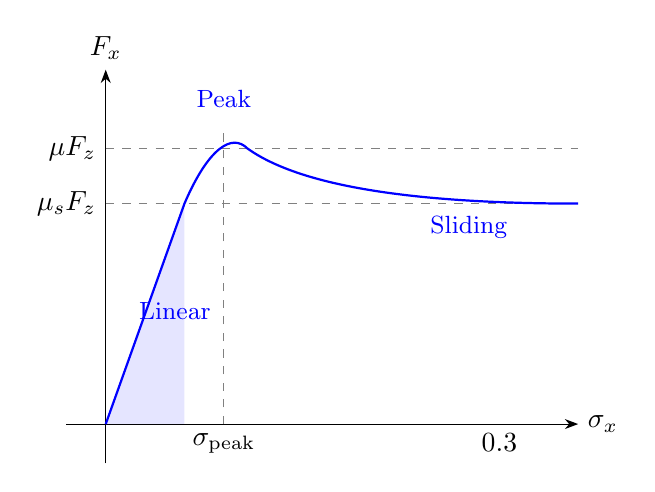
\begin{tikzpicture}[scale=1.0]
    % Axes
    \draw[-{Stealth}] (-0.5, 0) -- (6, 0) node[right] {$\sigma_x$};
    \draw[-{Stealth}] (0, -0.5) -- (0, 4.5) node[above] {$F_x$};
    
    % Labels on axes
    \node[below] at (1.5, 0) {$\sigma_{\text{peak}}$};
    \node[below] at (5, 0) {0.3};
    \node[left] at (0, 3.5) {$\mu F_z$};
    \node[left] at (0, 2.8) {$\mu_s F_z$};
    
    % Reference lines
    \draw[dashed, gray] (0, 3.5) -- (6, 3.5);
    \draw[dashed, gray] (0, 2.8) -- (6, 2.8);
    \draw[dashed, gray] (1.5, 0) -- (1.5, 3.7);
    
    % Dugoff curve
    \draw[thick, blue] (0, 0) -- (1.0, 2.8) 
        .. controls (1.3, 3.5) and (1.6, 3.7) .. (1.8, 3.5)
        .. controls (2.5, 3.0) and (4.0, 2.8) .. (6, 2.8);
    
    % Annotations
    \node[blue, above right] at (0.3, 1.2) {\small Linear};
    \node[blue, above] at (1.5, 3.9) {\small Peak};
    \node[blue, right] at (4.0, 2.5) {\small Sliding};
    
    % Fill linear region
    \fill[blue, opacity=0.1] (0, 0) -- (1.0, 2.8) -- (1.0, 0) -- cycle;
    
\end{tikzpicture}
\caption{Dugoff slip-force characteristic showing linear region, peak grip, and sliding region}
\label{fig:slip_force}
\end{figure}

%=============================================================================
\section{Wheel Rotational Dynamics}
\label{sec:wheel_dynamics}
%=============================================================================

This section introduces the key addition for the hybrid model: independent wheel speed integration.

\subsection{Motivation}

In the torque-only model, wheel speed is derived from vehicle speed:
\begin{equation}
\omega = \frac{V_x}{R} \quad \Rightarrow \quad \sigma_x = 0 \text{ always!}
\end{equation}

This prevents modeling of:
\begin{itemize}
    \item Wheel spin during aggressive acceleration
    \item Wheel lock during hard braking
    \item Natural slip development
    \item TCS/ABS algorithm testing
\end{itemize}

The solution is to integrate wheel angular velocity independently.

\subsection{Single Wheel Free Body Diagram}

For each wheel, applying Newton's second law for rotation:

\begin{equation}
\boxed{I_w \dot{\omega} = \tau_{\text{drive}} - \tau_{\text{brake}} - F_x \cdot R}
\label{eq:wheel_dynamics}
\end{equation}

where:
\begin{itemize}
    \item $I_w$ = wheel rotational inertia (kg$\cdot$m$^2$)
    \item $\omega$ = wheel angular velocity (rad/s)
    \item $\dot{\omega}$ = wheel angular acceleration (rad/s$^2$)
    \item $\tau_{\text{drive}}$ = drive torque at wheel (N$\cdot$m)
    \item $\tau_{\text{brake}}$ = brake torque (N$\cdot$m), always $\geq 0$
    \item $F_x$ = longitudinal tire force from Dugoff (N)
    \item $R$ = tire effective rolling radius (m)
\end{itemize}

\subsection{Drive Torque Distribution}

For a rear-wheel drive (RWD) configuration:

\begin{equation}
\tau_{\text{drive,rl}} = \tau_{\text{drive,rr}} = \frac{\tau_{\text{motor}} \cdot N_{\text{gear}} \cdot \eta_{\text{drivetrain}}}{2}
\end{equation}

\begin{equation}
\tau_{\text{drive,fl}} = \tau_{\text{drive,fr}} = 0 \quad \text{(front wheels not driven)}
\end{equation}

where:
\begin{itemize}
    \item $\tau_{\text{motor}}$ = motor shaft torque (N$\cdot$m)
    \item $N_{\text{gear}}$ = final drive gear ratio (dimensionless)
    \item $\eta_{\text{drivetrain}}$ = drivetrain efficiency (typically 0.90-0.95)
\end{itemize}

\subsection{Wheel Inertia}

The wheel rotational inertia includes:
\begin{equation}
I_w = I_{\text{tire}} + I_{\text{rim}} + I_{\text{brake}} + I_{\text{hub}}
\end{equation}

Typical values:
\begin{itemize}
    \item Passenger car: $I_w \approx 1.5-3.0$ kg$\cdot$m$^2$
    \item Mining haul truck (XCMG XDE320): $I_w \approx 800-1500$ kg$\cdot$m$^2$
\end{itemize}

\subsection{Discrete-Time Integration}

Using forward Euler integration:

\begin{equation}
\omega[k+1] = \omega[k] + \frac{\Delta t}{I_w} \left( \tau_{\text{drive}} - \tau_{\text{brake}} \cdot \text{sgn}(\omega[k]) - F_x[k] \cdot R \right)
\label{eq:wheel_integration}
\end{equation}

\textbf{Wheel Lock Detection:}
\begin{equation}
\text{if } \omega[k] > 0 \text{ and } \omega[k+1] < 0 \text{ and } \tau_{\text{brake}} > 0: \quad \omega[k+1] = 0
\end{equation}

This prevents non-physical sign reversal during braking.

\subsection{Stability Criterion}

The explicit integration is stable when:
\begin{equation}
\Delta t < \frac{2 I_w}{C_x R^2}
\end{equation}

For XCMG XDE320 parameters ($I_w = 1000$ kg$\cdot$m$^2$, $C_x = 280{,}000$ N, $R = 1.93$ m):
\begin{equation}
\Delta t_{\max} \approx \frac{2 \times 1000}{280{,}000 \times 1.93^2} \approx 1.9 \text{ ms}
\end{equation}

Simulation timestep of 1 ms provides adequate stability margin.

%=============================================================================
\section{Closed-Loop System Architecture}
\label{sec:closed_loop}
%=============================================================================

\subsection{System Block Diagram}

The hybrid model forms a closed-loop system:

\begin{figure}[H]
\centering
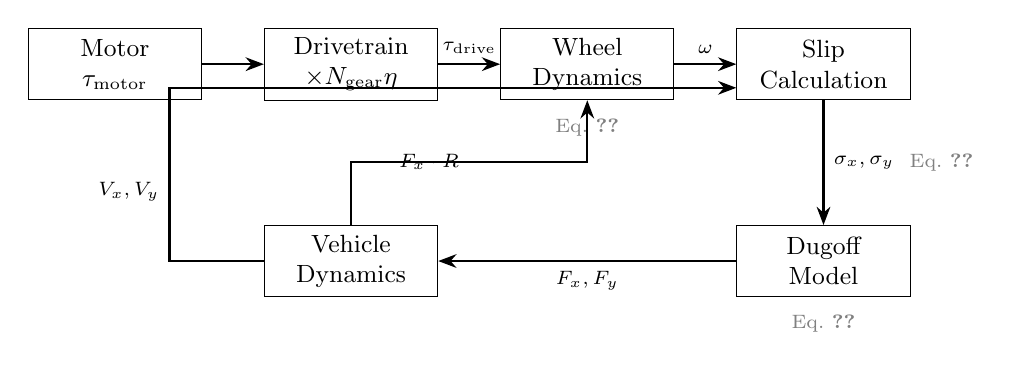
\begin{tikzpicture}[
    block/.style={rectangle, draw, minimum width=2.2cm, minimum height=0.9cm, align=center, font=\small},
    sum/.style={circle, draw, minimum size=0.4cm},
    arrow/.style={-{Stealth[scale=1.0]}, thick}
]

% Blocks - Top row
\node[block] (motor) at (0, 0) {Motor\\$\tau_{\text{motor}}$};
\node[block] (drivetrain) at (3, 0) {Drivetrain\\$\times N_{\text{gear}} \eta$};
\node[block] (wheel) at (6, 0) {Wheel\\Dynamics};
\node[block] (slip) at (9, 0) {Slip\\Calculation};

% Blocks - Bottom row
\node[block] (dugoff) at (9, -2.5) {Dugoff\\Model};
\node[block] (vehicle) at (3, -2.5) {Vehicle\\Dynamics};

% Arrows - Top row
\draw[arrow] (motor) -- (drivetrain);
\draw[arrow] (drivetrain) -- (wheel) node[midway, above, font=\scriptsize] {$\tau_{\text{drive}}$};
\draw[arrow] (wheel) -- (slip) node[midway, above, font=\scriptsize] {$\omega$};

% Arrows - Right side
\draw[arrow] (slip) -- (dugoff) node[midway, right, font=\scriptsize] {$\sigma_x, \sigma_y$};

% Arrows - Bottom
\draw[arrow] (dugoff) -- (vehicle) node[midway, below, font=\scriptsize] {$F_x, F_y$};

% Feedback arrows
\draw[arrow] (vehicle.north) -- ++(0, 0.8) -| (wheel.south) node[pos=0.25, left, font=\scriptsize] {$F_x \cdot R$};
\draw[arrow] (vehicle.west) -- ++(-1.2, 0) |- ($(slip.west) + (0, -0.3)$) node[pos=0.2, left, font=\scriptsize] {$V_x, V_y$};

% Equation labels
\node[font=\scriptsize, gray] at (6, -0.8) {Eq.~\ref{eq:wheel_dynamics}};
\node[font=\scriptsize, gray] at (10.5, -1.25) {Eq.~\ref{eq:slip_ratio}};
\node[font=\scriptsize, gray] at (9, -3.3) {Eq.~\ref{eq:Fx_dugoff}};

\end{tikzpicture}
\caption{Closed-loop system architecture for hybrid torque-slip model}
\label{fig:closed_loop}
\end{figure}

\subsection{Causality Chain}

At each timestep $k$:

\begin{enumerate}
    \item \textbf{Input:} Motor torque command $\tau_{\text{motor}}$
    \item \textbf{Drivetrain:} $\tau_{\text{wheel}} = \tau_{\text{motor}} \cdot N_{\text{gear}} \cdot \eta$
    \item \textbf{Wheel dynamics:} Integrate $\omega[k+1]$ using Eq.~\ref{eq:wheel_integration}
    \item \textbf{Slip calculation:} Compute $\sigma_x, \sigma_y$ using Eq.~\ref{eq:slip_ratio}
    \item \textbf{Dugoff model:} Compute $F_x, F_y$ using Eq.~\ref{eq:Fx_dugoff}, \ref{eq:Fy_dugoff}
    \item \textbf{Vehicle dynamics:} Update $V_x, V_y$ from tire forces
    \item \textbf{Feedback:} Tire reaction torque $F_x \cdot R$ affects next wheel integration
\end{enumerate}

\subsection{Key Insight: Feedback Loop}

The tire force $F_x$ appears on \textbf{both sides} of the system:
\begin{itemize}
    \item \textbf{Output:} Accelerates the vehicle ($m\dot{V}_x = \sum F_x$)
    \item \textbf{Feedback:} Decelerates the wheel ($I_w \dot{\omega} = \tau - F_x R$)
\end{itemize}

This creates natural self-regulation:
\begin{itemize}
    \item High slip $\rightarrow$ reduced $F_x$ (saturation) $\rightarrow$ wheel accelerates less
    \item Low slip $\rightarrow$ high $F_x$ $\rightarrow$ wheel slows toward free-rolling
\end{itemize}

%=============================================================================
\section{Lateral Velocity Computation}
%=============================================================================

\subsection{Front Axle Lateral Velocity}

Lateral velocity at front tire contact patch:
\begin{equation}
V_{y,\text{front}} = V_y + \dot{\psi} \cdot L_f - V_x \tan(\delta)
\end{equation}

where:
\begin{itemize}
    \item $V_y$ -- vehicle lateral velocity at CoG (m/s)
    \item $\dot{\psi}$ -- yaw rate (rad/s)
    \item $\delta$ -- steering angle (rad)
\end{itemize}

\subsection{Rear Axle Lateral Velocity}

\begin{equation}
V_{y,\text{rear}} = V_y - \dot{\psi} \cdot L_r
\end{equation}

\subsection{Lateral Slip Ratio per Wheel}

\begin{align}
\sigma_{y,\text{fl}} = \sigma_{y,\text{fr}} &= \frac{V_{y,\text{front}}}{V_x} \\
\sigma_{y,\text{rl}} = \sigma_{y,\text{rr}} &= \frac{V_{y,\text{rear}}}{V_x}
\end{align}

%=============================================================================
\section{Torque-Only vs Hybrid Model}
\label{sec:comparison}
%=============================================================================

\subsection{Torque-Only Model (Current Default)}

Direct force computation without wheel dynamics:
\begin{equation}
F_x = \min\left( \frac{\tau_{\text{motor}} \cdot N_{\text{gear}} \cdot \eta}{R}, \mu F_z \right)
\end{equation}

\textbf{Advantages:}
\begin{itemize}
    \item Simple, fast computation
    \item No additional state variables
    \item Stable at all speeds
    \item Captures traction limiting
\end{itemize}

\textbf{Limitations:}
\begin{itemize}
    \item Cannot model wheel spin ($\omega \gg V_x/R$)
    \item Cannot model wheel lock ($\omega = 0$ while $V_x > 0$)
    \item Slip ratio is estimated, not computed
    \item No TCS/ABS testing capability
\end{itemize}

\subsection{Hybrid Model}

Full causality: $\tau_{\text{motor}} \rightarrow \omega \rightarrow \sigma_x \rightarrow F_x$

\textbf{Advantages:}
\begin{itemize}
    \item Physical wheel spin and lock behavior
    \item Natural slip development
    \item Full Dugoff slip-force curve (including peak and sliding)
    \item TCS/ABS algorithm testing
    \item Realistic launch and braking dynamics
\end{itemize}

\textbf{Limitations:}
\begin{itemize}
    \item Additional state variables (4 wheel speeds)
    \item Requires smaller timestep for stability
    \item More complex initialization
\end{itemize}

\subsection{Model Selection Guide}

\begin{table}[H]
\centering
\begin{tabular}{lcc}
\toprule
\textbf{Use Case} & \textbf{Torque-Only} & \textbf{Hybrid} \\
\midrule
Path following & $\checkmark$ & $\checkmark$ \\
Energy estimation & $\checkmark$ & $\checkmark$ \\
Traction limiting & $\checkmark$ & $\checkmark$ \\
Wheel spin detection & & $\checkmark$ \\
ABS/TCS development & & $\checkmark$ \\
Stability control & & $\checkmark$ \\
Loss of control & & $\checkmark$ \\
\bottomrule
\end{tabular}
\caption{Model selection based on use case}
\end{table}

%=============================================================================
\section{Implementation Algorithm}
%=============================================================================

\subsection{Torque-Only Algorithm}

\textbf{Step 1: Compute Normal Loads}
\begin{enumerate}
    \item Static distribution from geometry
    \item Load transfer: $\Delta F_z = m a_x h_{\text{cg}} / L$
    \item Per-wheel loads
\end{enumerate}

\textbf{Step 2: Compute Demanded Force}
\begin{equation}
F_{x,\text{demanded}} = \frac{\tau_{\text{motor}} \cdot N_{\text{gear}} \cdot \eta}{R}
\end{equation}

\textbf{Step 3: Apply Friction Limit}
\begin{equation}
F_x = \min(|F_{x,\text{demanded}}|, \mu F_z) \cdot \text{sgn}(F_{x,\text{demanded}})
\end{equation}

\textbf{Step 4: Update Vehicle Dynamics}
\begin{equation}
a = \frac{\sum F_x - F_{\text{drag}} - F_{\text{roll}}}{m}
\end{equation}

\subsection{Hybrid Algorithm}

\textbf{Step 1: Compute Normal Loads} (same as torque-only)

\textbf{Step 2: Compute Slip Ratios from Current Wheel Speeds}
\begin{equation}
\sigma_x = \frac{\omega R - V_x}{\max(|V_x|, |\omega R|, V_{\min})}
\end{equation}

\textbf{Step 3: Compute Tire Forces (Dugoff)}
\begin{align}
\lambda &= \frac{\mu F_z}{2\sqrt{(C_x \sigma_x)^2 + (C_y \sigma_y)^2}} \\
f(\lambda) &= \begin{cases} (2-\lambda)\lambda & \lambda < 1 \\ 1 & \lambda \geq 1 \end{cases} \\
F_x &= C_x \sigma_x f(\lambda)
\end{align}

\textbf{Step 4: Update Wheel Dynamics}
\begin{equation}
\omega[k+1] = \omega[k] + \frac{\Delta t}{I_w}(\tau_{\text{drive}} - \tau_{\text{brake}} \cdot \text{sgn}(\omega) - F_x R)
\end{equation}

\textbf{Step 5: Update Vehicle Dynamics}
\begin{equation}
V_x[k+1] = V_x[k] + \frac{\Delta t}{m}(\sum F_x - F_{\text{drag}} - F_{\text{roll}})
\end{equation}

\subsection{Complete Discrete-Time State Update}

\begin{align}
\omega_i[k+1] &= \omega_i[k] + \Delta t \cdot \dot{\omega}_i \quad \text{(for each wheel $i$)} \\
V_x[k+1] &= V_x[k] + \Delta t \cdot a_x \\
\dot{\psi}[k] &= \frac{V_x[k]}{L} \tan(\delta[k]) \quad \text{(or from lateral dynamics)} \\
\psi[k+1] &= \psi[k] + \Delta t \cdot \dot{\psi}[k] \\
x[k+1] &= x[k] + \Delta t \cdot V_x[k] \cos(\psi[k]) \\
y[k+1] &= y[k] + \Delta t \cdot V_x[k] \sin(\psi[k])
\end{align}

%=============================================================================
\section{Surface Friction Coefficients}
%=============================================================================

\subsection{Mining Haul Road Conditions}

\begin{table}[H]
\centering
\begin{tabular}{lcc}
\toprule
\textbf{Surface} & $\mu_{\text{peak}}$ & $\mu_{\text{slide}}$ \\
\midrule
Dry pavement & 0.85 & 0.70 \\
Compact gravel & 0.72 & 0.60 \\
Loose gravel & 0.55 & 0.45 \\
Iron ore dust (dry) & 0.45 & 0.35 \\
Iron ore dust (wet) & 0.30 & 0.22 \\
Mud & 0.25 & 0.18 \\
Sand (loose) & 0.40 & 0.32 \\
\bottomrule
\end{tabular}
\caption{Friction coefficients for Pilbara mining conditions}
\end{table}

\subsection{Effect of Surface Friction}

The surface friction $\mu$ directly affects:

\begin{enumerate}
    \item \textbf{Maximum traction force:} $F_{x,\max} = \mu F_z$
    \item \textbf{Maximum acceleration:} $a_{\max} = \mu g$ (flat road)
    \item \textbf{Stopping distance:} $d_{\text{stop}} = \frac{v_0^2}{2\mu g}$
    \item \textbf{Friction utilization:} Lower $\mu$ means earlier saturation ($\lambda < 1$)
\end{enumerate}

%=============================================================================
\section{Implementation Parameters}
%=============================================================================

\subsection{XCMG XDE320 Mining Truck}

\begin{table}[H]
\centering
\begin{tabular}{lll}
\toprule
\textbf{Parameter} & \textbf{Value} & \textbf{Unit} \\
\midrule
Mass (empty) & 218,000 & kg \\
Mass (loaded) & 538,000 & kg \\
Wheelbase $L$ & 6.3 & m \\
Track width $W$ & 4.0 & m \\
CG height $h_{\text{cg}}$ & 2.8 & m \\
Tire radius $R$ & 1.93 & m \\
Gear ratio $N_{\text{gear}}$ & 9.0 & - \\
Drivetrain efficiency $\eta$ & 0.92 & - \\
Motor max torque & 145,000 & N$\cdot$m \\
Motor max power & 2,100 & kW \\
\bottomrule
\end{tabular}
\caption{Vehicle parameters}
\end{table}

\begin{table}[H]
\centering
\begin{tabular}{lll}
\toprule
\textbf{Parameter} & \textbf{Value} & \textbf{Unit} \\
\midrule
$C_{x,\text{base}}$ & 280,000 & N \\
$C_{y,\text{base}}$ & 220,000 & N \\
$F_{z,\text{ref}}$ & 100,000 & N \\
$I_w$ (front) & 800 & kg$\cdot$m$^2$ \\
$I_w$ (rear) & 1,200 & kg$\cdot$m$^2$ \\
\bottomrule
\end{tabular}
\caption{Tire and wheel parameters}
\end{table}

%=============================================================================
\section{Validation and Benchmarks}
%=============================================================================

\subsection{Expected Behavior}

\textbf{Scenario 1: Acceleration on gravel ($\mu = 0.72$)}

XCMG XDE320 empty (218 tons):
\begin{align}
F_{z,\text{rear}} &\approx 0.60 \times 218{,}000 \times 9.81 = 1{,}283{,}000 \text{ N} \\
F_{x,\text{max}} &= 0.72 \times 1{,}283{,}000 = 924{,}000 \text{ N} \\
a_{\max} &= \frac{924{,}000}{218{,}000} = 4.2 \text{ m/s}^2
\end{align}

\textbf{Scenario 2: Acceleration on wet dust ($\mu = 0.30$)}

\begin{align}
F_{x,\text{max}} &= 0.30 \times 1{,}283{,}000 = 385{,}000 \text{ N} \\
a_{\max} &= \frac{385{,}000}{218{,}000} = 1.8 \text{ m/s}^2
\end{align}

\textbf{Result:} Acceleration limited to 1.8 m/s$^2$ on wet dust vs 4.2 m/s$^2$ on gravel.

\subsection{Stopping Distance Comparison}

For $v_0 = 50$ km/h = 13.9 m/s:

\begin{align}
d_{\text{gravel}} &= \frac{13.9^2}{2 \times 0.72 \times 9.81} = 13.7 \text{ m} \\
d_{\text{wet dust}} &= \frac{13.9^2}{2 \times 0.30 \times 9.81} = 32.8 \text{ m}
\end{align}

Stopping distance increases 2.4$\times$ on wet dust compared to gravel.

%=============================================================================
\section{Future Enhancements}
%=============================================================================

\subsection{Short-Term (V2.5)}
\begin{itemize}
    \item[$\checkmark$] Wheel rotational dynamics (this document)
    \item[$\checkmark$] Hybrid torque-slip model
    \item Combined longitudinal-lateral friction circle
\end{itemize}

\subsection{Medium-Term (V3)}
\begin{itemize}
    \item 3-DOF vehicle dynamics (add $V_y$, $\dot{\psi}$ as states)
    \item Oversteer/understeer simulation
    \item Loss of control scenarios
\end{itemize}

\subsection{Long-Term (V4)}
\begin{itemize}
    \item 6-DOF dynamics (roll, pitch, heave)
    \item Suspension dynamics
    \item Rollover detection and prevention
\end{itemize}

%=============================================================================
\section{Conclusion}
%=============================================================================

This document presents a comprehensive vehicle dynamics model with two levels of tire modeling:

\textbf{Torque-Only Model:}
\begin{itemize}
    \item Simple friction-limited force calculation
    \item Suitable for energy estimation and path following
    \item Cannot model wheel spin or lock
\end{itemize}

\textbf{Hybrid Torque-Slip Model:}
\begin{itemize}
    \item Independent wheel speed integration
    \item Natural slip development
    \item Full Dugoff slip-force characteristic
    \item Enables TCS/ABS/ESC development
\end{itemize}

Both models share:
\begin{itemize}
    \item Load transfer during acceleration/braking
    \item Surface friction effects
    \item Friction circle constraint
\end{itemize}

This forms a solid foundation for autonomous mining vehicle simulation.

%=============================================================================
\begin{thebibliography}{9}

\bibitem{dugoff1970}
Dugoff, H., Fancher, P. S., and Segel, L. (1970).
\textit{An Analysis of Tire Traction Properties and Their Influence on Vehicle Dynamic Performance}.
SAE Technical Paper 700377.

\bibitem{rajamani2012}
Rajamani, R. (2012). \textit{Vehicle Dynamics and Control}. Springer.

\bibitem{gillespie1992}
Gillespie, T. D. (1992). \textit{Fundamentals of Vehicle Dynamics}. SAE International.

\bibitem{pacejka2012}
Pacejka, H. (2012). \textit{Tire and Vehicle Dynamics}, 3rd Edition. Butterworth-Heinemann.

\bibitem{iso8855}
ISO 8855:2011. Road vehicles -- Vehicle dynamics and road-holding ability -- Vocabulary.

\end{thebibliography}

\end{document}